\documentclass[12pt,a4paper]{article}

% -------------------------------------------------
% PACKAGES
% -------------------------------------------------
\usepackage[a4paper,margin=1in]{geometry}
\usepackage{graphicx}
\usepackage{booktabs}
\usepackage{amsmath,amssymb}
\usepackage{float}
\usepackage{hyperref}
\usepackage{xcolor}
\usepackage{listings}
\usepackage{enumitem}
\usepackage{fancyhdr}
\usepackage{longtable}
\usepackage{array}

% -------------------------------------------------
% HYPERLINK SETTINGS
% -------------------------------------------------
\hypersetup{
    colorlinks=true,
    linkcolor=blue,
    urlcolor=blue
}

% -------------------------------------------------
% HEADER AND FOOTER
% -------------------------------------------------
\pagestyle{fancy}
\fancyhf{}
\lhead{ICS1512}
\rhead{Machine Learning Algorithms Laboratory}
\cfoot{\thepage}

% -------------------------------------------------
% PYTHON CODE SETTINGS
% -------------------------------------------------
\definecolor{codegreen}{rgb}{0,0.45,0}
\definecolor{codegray}{rgb}{0.45,0.45,0.45}
\definecolor{codeblue}{rgb}{0.0,0.2,0.6}

\lstset{
    language=Python,
    basicstyle=\ttfamily\footnotesize,
    numbers=left,
    numberstyle=\tiny\color{codegray},
    frame=single,
    breaklines=true,
    showstringspaces=false,
    keywordstyle=\color{codeblue},
    commentstyle=\color{codegreen},
    stringstyle=\color{codeblue},
    columns=fullflexible
}

% -------------------------------------------------
% DOCUMENT
% -------------------------------------------------
\begin{document}

% =================================================
% TITLE PAGE / EXPERIMENT DETAILS
% =================================================

\begin{center}
    {\Large\textbf{Machine Learning Algorithms Laboratory}}\\[0.3cm]
    {\large\textbf{Experiment 2}}\\[0.2cm]
    {\Large\textbf{Email Spam/Ham Classification using Naive Bayes and KNN}}
\end{center}

\vspace{0.5cm}

\begin{tabular}{|p{4cm}|p{10.5cm}|}
\hline
\textbf{Experiment No.} & 2 \\ \hline

\textbf{Experiment Title} &
Email Spam/Ham Classification using Naive Bayes and KNN \\ \hline

\textbf{Student Name} &
Harshitaa B \\ \hline

\textbf{Register Number} &
3122247001021 \\ \hline

\textbf{Faculty} &
Dr. Poreddy Ajay Kumar Reddy \\ \hline

\textbf{Submission Date} &
16th August 2026 \\ \hline

\end{tabular}

% =================================================
% OBJECTIVE
% =================================================

\section{Objective}

The objective of this experiment is to classify emails into spam and ham categories using different machine learning algorithms. Naive Bayes and K-Nearest Neighbour (KNN) classifiers are implemented and evaluated using standard classification metrics.

The experiment also aims to:

\begin{itemize}
    \item Compare Gaussian, Multinomial and Bernoulli Naive Bayes.
    \item Study the effect of different values of $k$ in KNN.
    \item Compare KNN performance for different neighbourhood sizes.
    \item Perform hyperparameter tuning using GridSearchCV and RandomizedSearchCV.
    \item Compare KDTree and BallTree for nearest-neighbour search.
    \item Perform five-fold cross-validation.
    \item Compare training and prediction time.
\end{itemize}

% =================================================
% PROBLEM STATEMENT
% =================================================

\section{Problem Statement}

The task is to classify email messages into two classes: spam and ham. The dataset contains numerical features extracted from email messages.

A classification model is trained using the available labelled data and then used to predict the class of previously unseen emails.

The performance of the models is evaluated using:

\begin{itemize}
    \item Accuracy
    \item Precision
    \item Recall
    \item F1-score
    \item ROC-AUC
\end{itemize}

% =================================================
% DATASET
% =================================================

\section{Dataset Description}

The experiment uses the Spambase dataset.

\begin{longtable}{|p{6cm}|p{8cm}|}
\hline
\textbf{Dataset Property} & \textbf{Description} \\ \hline

Dataset Name & Spambase \\ \hline

Number of Samples & 4601 \\ \hline

Number of Features & 57 \\ \hline

Number of Classes & 2 \\ \hline

Target Variable & class \\ \hline

Class 0 & Ham \\ \hline

Class 1 & Spam \\ \hline

Train-Test Split & 80:20 stratified split \\ \hline

Missing Values & Checked during preprocessing \\ \hline

\end{longtable}

% =================================================
% EDA
% =================================================

\section{Exploratory Data Analysis}

Exploratory Data Analysis was performed before model training to understand the structure and characteristics of the dataset.

The following aspects were examined:

\begin{itemize}
    \item Dataset dimensions
    \item Statistical summary
    \item Missing values
    \item Class distribution
    \item Correlation between features
    \item Feature distributions
\end{itemize}

% -------------------------------------------------
% CLASS DISTRIBUTION
% -------------------------------------------------

\subsection{Class Distribution}

\begin{figure}[H]
\centering
\IfFileExists{figs/class_distribution.png}
{
    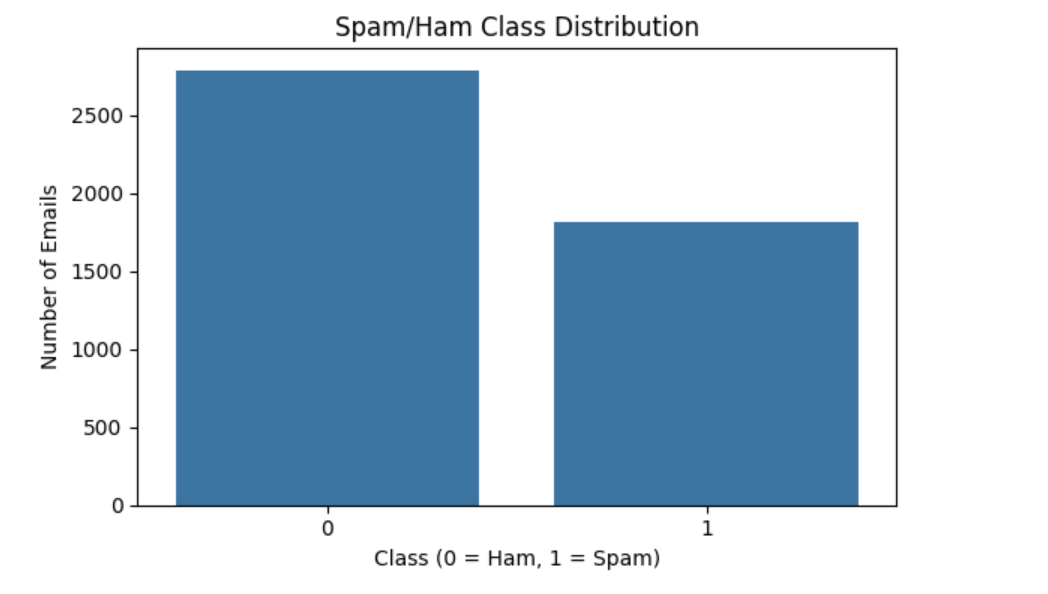
\includegraphics[width=0.75\linewidth]{figs/class_distribution.png}
}
{
    \fbox{
    \parbox[c][4cm][c]{0.7\linewidth}{
    \centering
    Insert class distribution graph here
    }}
}
\caption{Distribution of spam and ham emails}
\end{figure}

\textbf{Observation:}

The class distribution graph shows the number of spam and ham emails present in the dataset. The two classes are not perfectly balanced, so accuracy alone may not completely describe the classification performance. Therefore, precision, recall, F1-score and ROC-AUC are also considered.

% -------------------------------------------------
% CORRELATION
% -------------------------------------------------

\subsection{Correlation Matrix}

\begin{figure}[H]
\centering
\IfFileExists{figs/correlation_matrix.png}
{
    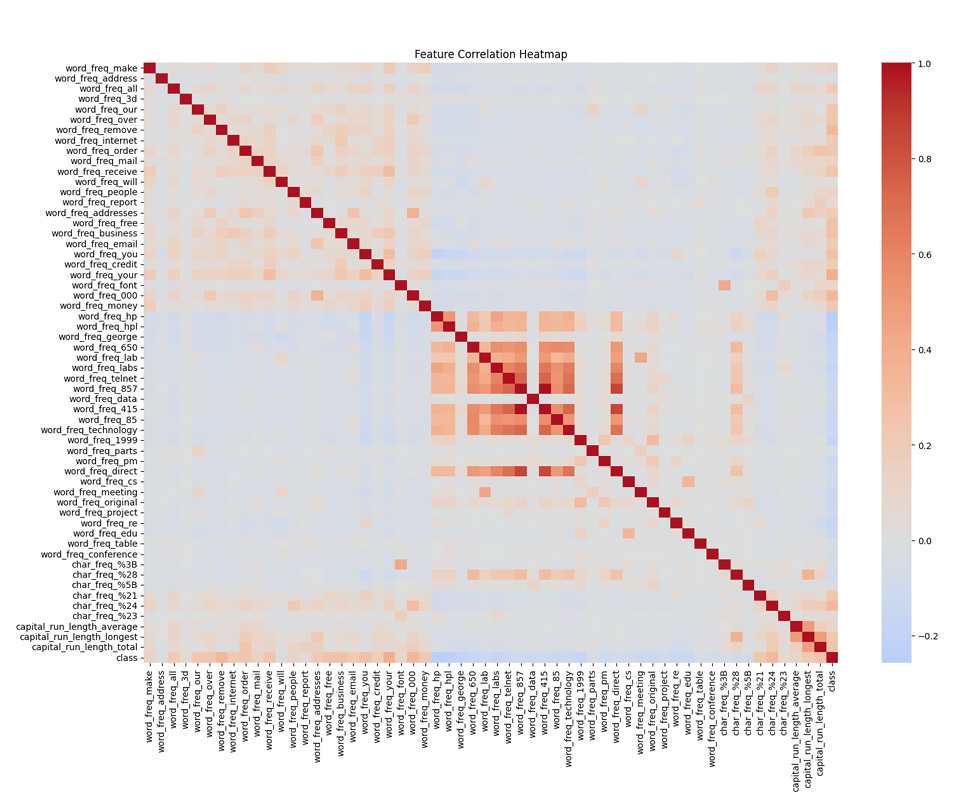
\includegraphics[width=0.85\linewidth]{figs/correlation_matrix.png}
}
{
    \fbox{
    \parbox[c][4cm][c]{0.7\linewidth}{
    \centering
    Insert correlation heatmap here
    }}
}
\caption{Correlation matrix of dataset features}
\end{figure}

\textbf{Observation:}

The correlation matrix represents the relationship between different numerical features. The diagonal elements have a correlation value of one because each feature is perfectly correlated with itself. Some features show stronger relationships with each other, while many feature pairs have relatively weak correlation.

% -------------------------------------------------
% FEATURE DISTRIBUTION
% -------------------------------------------------

\subsection{Feature Distribution}

\begin{figure}[H]
\centering
\IfFileExists{figs/feature_distribution_1.png}
{
    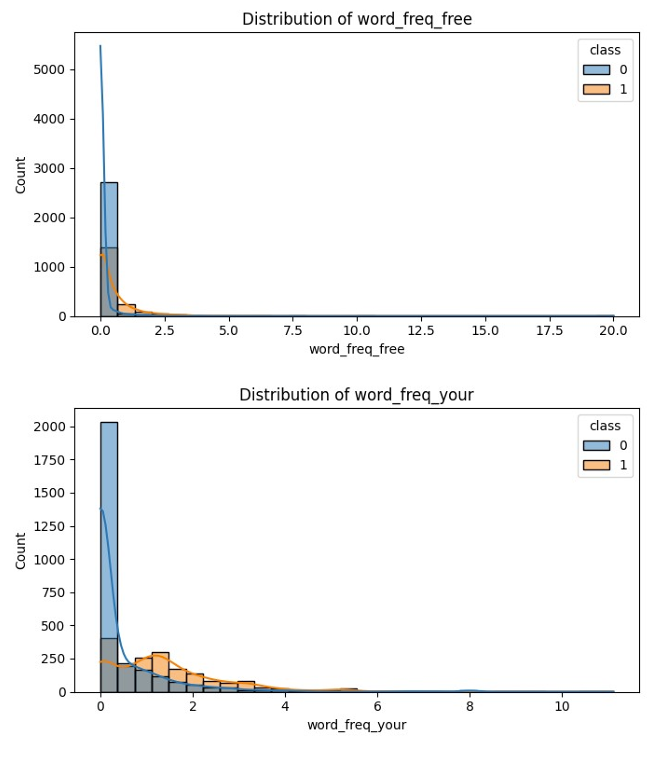
\includegraphics[width=0.85\linewidth]{figs/feature_distribution_1.png}
}
{
    \fbox{
    \parbox[c][4cm][c]{0.7\linewidth}{
    \centering
    Insert feature distribution graph here
    }}
}
\caption{Distribution of selected features}
\end{figure}

\begin{figure}[H]
\centering
\IfFileExists{figs/feature_distribution_2.png}
{
    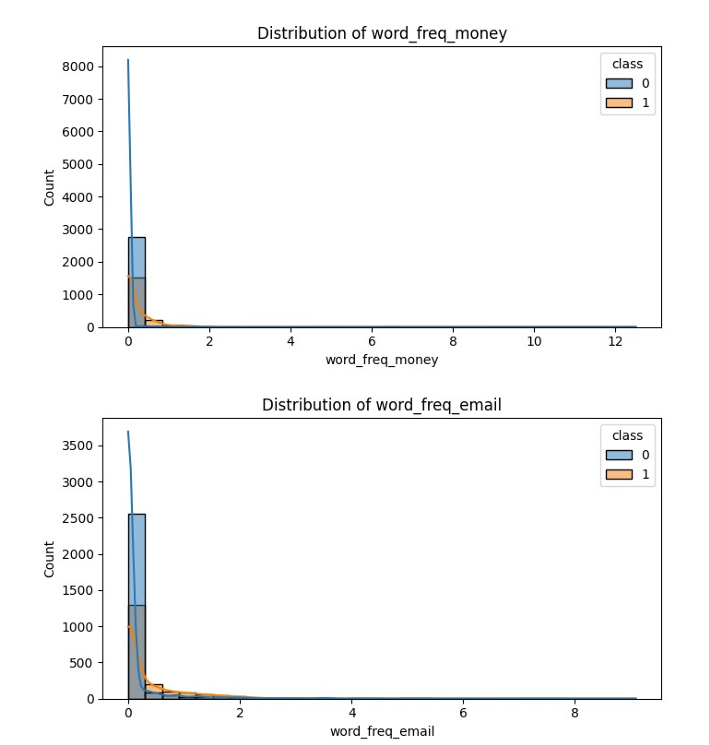
\includegraphics[width=0.85\linewidth]{figs/feature_distribution_2.png}
}
{
    \fbox{
    \parbox[c][4cm][c]{0.7\linewidth}{
    \centering
    Insert feature distribution graph here
    }}
}
\caption{Distribution of selected features}
\end{figure}

\textbf{Observation:}

The feature distribution plots show how the values of selected features are distributed across the dataset. Some features are concentrated near zero, while a smaller number of observations contain relatively larger values. Such differences in distributions can provide useful information for distinguishing spam from ham emails.

% =================================================
% PREPROCESSING
% =================================================

\section{Data Preprocessing}

The following preprocessing operations were performed:

\begin{enumerate}
    \item The dataset was loaded using Pandas.
    \item The dataset was checked for missing values.
    \item The target variable was separated from the input features.
    \item The dataset was divided into training and testing sets.
    \item Stratification was used to maintain the class distribution.
    \item Feature scaling was applied where required.
\end{enumerate}

For KNN, feature scaling is important because the algorithm uses distances between samples.

Standardization was performed using:

\[
z = \frac{x-\mu}{\sigma}
\]

where $x$ is the original feature value, $\mu$ is the mean and $\sigma$ is the standard deviation.

% =================================================
% MACHINE LEARNING ALGORITHMS
% =================================================

\section{Machine Learning Algorithms}

% -------------------------------------------------
% NAIVE BAYES
% -------------------------------------------------

\subsection{Naive Bayes}

Naive Bayes is a probabilistic classification algorithm based on Bayes' theorem.

\[
P(C|X)=\frac{P(X|C)P(C)}{P(X)}
\]

where:

\begin{itemize}
    \item $C$ represents the class.
    \item $X$ represents the input feature vector.
    \item $P(C|X)$ is the posterior probability.
    \item $P(X|C)$ is the likelihood.
    \item $P(C)$ is the prior probability.
\end{itemize}

The three variants considered in this experiment are:

\begin{itemize}
    \item Gaussian Naive Bayes
    \item Multinomial Naive Bayes
    \item Bernoulli Naive Bayes
\end{itemize}

% -------------------------------------------------
% KNN
% -------------------------------------------------

\subsection{K-Nearest Neighbour}

KNN classifies a new sample according to the classes of its nearest training samples.

The Minkowski distance is given by:

\[
d(x,y)=
\left(
\sum_{i=1}^{d}|x_i-y_i|^p
\right)^{1/p}
\]

For $p=1$, the distance corresponds to Manhattan distance.

For $p=2$, the distance corresponds to Euclidean distance.

Different values of $k$ were tested:

\[
k \in \{1,3,5,7,9,11\}
\]

% =================================================
% EXPERIMENTAL SETUP
% =================================================

\section{Experimental Setup}

\begin{tabular}{ll}
\toprule
Python Version & As used in the experiment \\
Scikit-Learn & As used in the experiment \\
IDE & Jupyter Notebook \\
Dataset & Spambase \\
Train-Test Split & 80:20 \\
Cross-Validation & 5-fold \\
\bottomrule
\end{tabular}

% =================================================
% NAIVE BAYES RESULTS
% =================================================

\section{Results}

\subsection{Naive Bayes Comparison}

\begin{longtable}{|p{3.5cm}|c|c|c|c|c|}
\hline
\textbf{Model} &
\textbf{Accuracy} &
\textbf{Precision} &
\textbf{Recall} &
\textbf{F1} &
\textbf{ROC-AUC} \\ \hline

Gaussian NB &
0.8328 &
0.7146 &
0.9587 &
0.8188 &
0.9376 \\ \hline

Multinomial NB &
0.8958 &
0.9349 &
0.7906 &
0.8567 &
0.9612 \\ \hline

Bernoulli NB &
0.8795 &
0.8684 &
0.8182 &
0.8426 &
0.9457 \\ \hline

\end{longtable}

\textbf{Observation:}

Among the three Naive Bayes models, Multinomial Naive Bayes achieved the highest accuracy of approximately 89.58\%. It also obtained the highest precision and ROC-AUC among the three Naive Bayes models. Gaussian Naive Bayes obtained the highest recall, meaning that it detected a larger proportion of spam samples, although its precision was lower.

% =================================================
% KNN RESULTS
% =================================================

\subsection{KNN Performance for Different Values of $k$}

\begin{longtable}{|c|c|c|c|c|c|}
\hline
$k$ &
Accuracy &
Precision &
Recall &
F1-score &
ROC-AUC \\ \hline

1 &
0.8990 &
0.8792 &
0.8623 &
0.8707 &
0.8926 \\ \hline

3 &
0.8979 &
0.8726 &
0.8678 &
0.8702 &
0.9360 \\ \hline

5 &
0.9077 &
0.8861 &
0.8788 &
0.8824 &
0.9506 \\ \hline

7 &
0.9088 &
0.8930 &
0.8733 &
0.8830 &
0.9566 \\ \hline

9 &
0.9088 &
0.8930 &
0.8733 &
0.8830 &
0.9602 \\ \hline

11 &
0.9099 &
0.9000 &
0.8678 &
0.8836 &
0.9622 \\ \hline

\end{longtable}

\textbf{Observation:}

The KNN model achieved its highest accuracy for $k=11$, with an accuracy of approximately 90.99\%. The F1-score was also highest at $k=11$. The ROC-AUC increased considerably as the value of $k$ increased, reaching 0.9622 for $k=11$. Therefore, $k=11$ was selected as the best value among the tested configurations.

% =================================================
% KNN GRAPH
% =================================================

\subsection{Accuracy versus $k$}

\begin{figure}[H]
\centering
\IfFileExists{figs/Accuracy_k.png}
{
    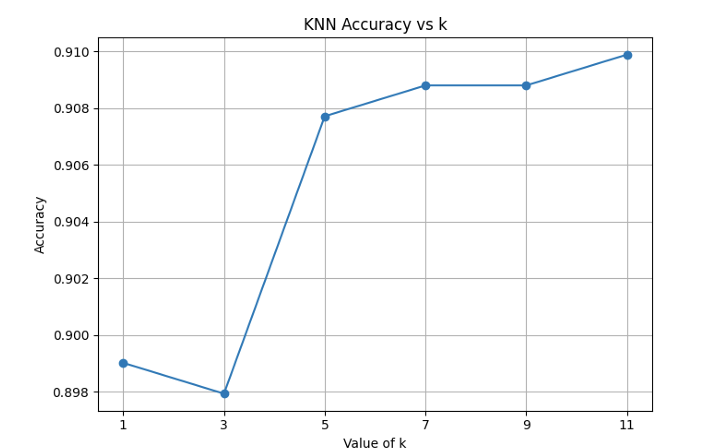
\includegraphics[width=0.75\linewidth]{figs/Accuracy_k.png}
}
{
    \fbox{
    \parbox[c][4cm][c]{0.7\linewidth}{
    \centering
    Insert KNN accuracy graph here
    }}
}
\caption{KNN accuracy for different values of $k$}
\end{figure}

\textbf{Inference:}

The accuracy generally improves as $k$ increases from 1 to 11. The highest accuracy is obtained at $k=11$. The small changes between $k=7$, $k=9$ and $k=11$ indicate that the model performance becomes relatively stable for larger neighbourhood sizes.

% =================================================
% CLASSIFIER COMPARISON
% =================================================

\subsection{Overall Classifier Comparison}

\begin{longtable}{|p{4cm}|c|c|c|c|c|}
\hline
\textbf{Model} &
\textbf{Accuracy} &
\textbf{Precision} &
\textbf{Recall} &
\textbf{F1} &
\textbf{ROC-AUC} \\ \hline

Gaussian NB &
0.8328 &
0.7146 &
0.9587 &
0.8188 &
0.9376 \\ \hline

Multinomial NB &
0.8958 &
0.9349 &
0.7906 &
0.8567 &
0.9612 \\ \hline

Bernoulli NB &
0.8795 &
0.8684 &
0.8182 &
0.8426 &
0.9457 \\ \hline

KNN ($k=11$) &
0.9099 &
0.9000 &
0.8678 &
0.8836 &
0.9622 \\ \hline

\end{longtable}

\textbf{Observation:}

KNN with $k=11$ achieved the highest accuracy among the compared models, with a value of approximately 90.99\%. It also achieved the highest F1-score and ROC-AUC. Multinomial Naive Bayes obtained the highest precision, while Gaussian Naive Bayes achieved the highest recall.

% =================================================
% KD TREE VS BALL TREE
% =================================================

\subsection{KDTree versus BallTree}

\begin{longtable}{|p{3.5cm}|c|c|c|}
\hline
\textbf{Algorithm} &
\textbf{Accuracy} &
\textbf{Training Time (s)} &
\textbf{Prediction Time (s)} \\ \hline

KDTree &
0.9099 &
0.03863 &
0.32900 \\ \hline

BallTree &
0.9099 &
0.02679 &
0.31920 \\ \hline

\end{longtable}

\textbf{Observation:}

Both KDTree and BallTree produced the same accuracy of approximately 90.99\%. BallTree required less training time and prediction time than KDTree in this experiment. The measured training time was approximately 0.0268 seconds for BallTree compared with 0.0386 seconds for KDTree. BallTree also had a slightly lower prediction time.

Therefore, BallTree was faster for the given dataset while maintaining the same classification accuracy.

% =================================================
% TIME RESULTS
% =================================================

\subsection{Training and Prediction Time}

\begin{longtable}{|p{4cm}|c|c|}
\hline
\textbf{Model} &
\textbf{Training Time (s)} &
\textbf{Prediction Time (s)} \\ \hline

Gaussian NB &
0.03763 &
0.02083 \\ \hline

Multinomial NB &
0.01725 &
0.01288 \\ \hline

Bernoulli NB &
0.02453 &
0.01223 \\ \hline

KNN ($k=11$) &
0.01034 &
0.22069 \\ \hline

\end{longtable}

\textbf{Observation:}

KNN required the least training time among the models listed, taking approximately 0.0103 seconds. However, its prediction time was significantly higher at approximately 0.2207 seconds. This is expected because KNN performs distance calculations during prediction rather than learning a complex parametric model during training.

Multinomial Naive Bayes also showed relatively low training and prediction times. Bernoulli Naive Bayes had the lowest prediction time among the Naive Bayes variants.

% =================================================
% CONFUSION MATRIX
% =================================================

\subsection{Confusion Matrix}

\begin{figure}[H]
\centering
\IfFileExists{figs/confusion_matrix_1.png}
{
    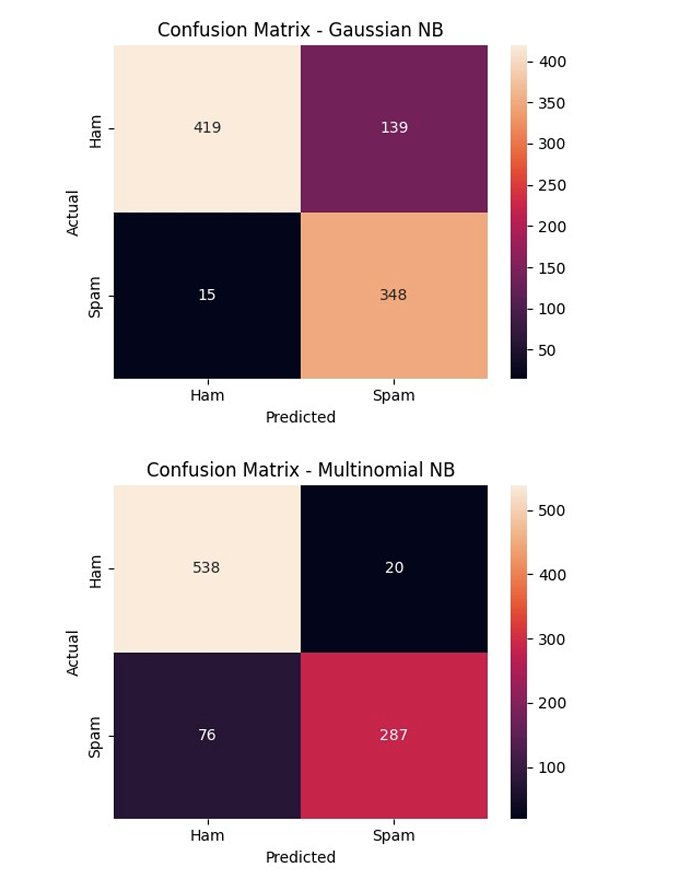
\includegraphics[width=0.70\linewidth]{figs/confusion_matrix_1.png}
}
{
    \fbox{
    \parbox[c][4cm][c]{0.7\linewidth}{
    \centering
    Insert confusion matrix here
    }}
}
\caption{Confusion matrix of the selected classifier}
\end{figure}


\begin{figure}[H]
\centering
\IfFileExists{figs/confusion_matrix_2.png}
{
    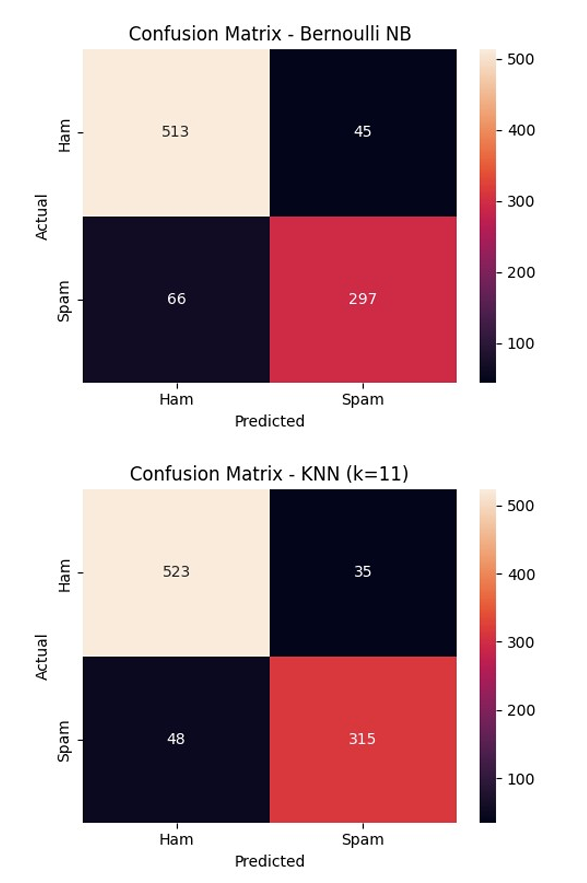
\includegraphics[width=0.70\linewidth]{figs/confusion_matrix_2.png}
}
{
    \fbox{
    \parbox[c][4cm][c]{0.7\linewidth}{
    \centering
    Insert confusion matrix here
    }}
}
\caption{Confusion matrix of the selected classifier}
\end{figure}
\textbf{Inference:}

The confusion matrix shows the number of correctly and incorrectly classified emails. The diagonal elements represent correct predictions, while the off-diagonal elements represent classification errors. The matrix provides a clearer view of false positives and false negatives than accuracy alone.

% =================================================
% ROC CURVE
% =================================================

\subsection{ROC Curve}

\begin{figure}[H]
\centering
\IfFileExists{figs/ROC_curves.png}
{
    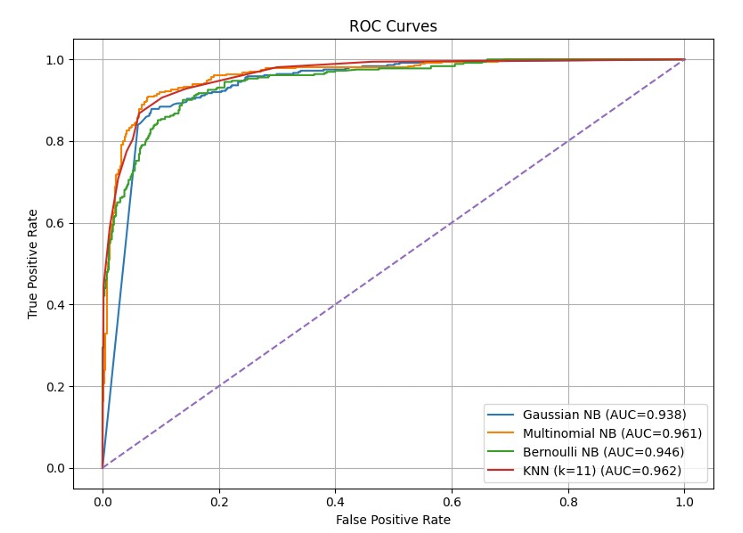
\includegraphics[width=0.75\linewidth]{figs/ROC_curves.png}
}
{
    \fbox{
    \parbox[c][4cm][c]{0.7\linewidth}{
    \centering
    Insert ROC curve here
    }}
}
\caption{ROC curves of the evaluated classifiers}
\end{figure}

\textbf{Inference:}

The ROC curve represents the relationship between the true positive rate and false positive rate for different classification thresholds. A curve closer to the upper-left corner indicates better classification performance. KNN with $k=11$ achieved the highest ROC-AUC among the compared models with a value of approximately 0.9622.

% =================================================
% PRECISION RECALL
% =================================================

\subsection{Precision-Recall Curve}

\begin{figure}[H]
\centering
\IfFileExists{figs/precision_recall_curves.png}
{
    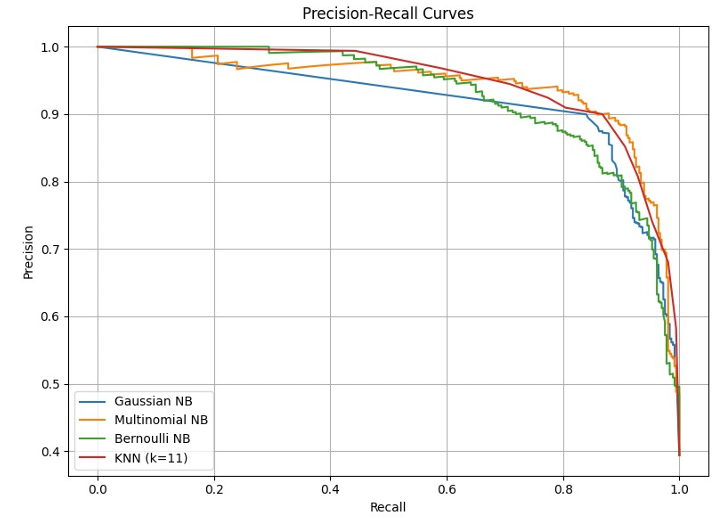
\includegraphics[width=0.75\linewidth]{figs/Precision_recall_curves.png}
}
{
    \fbox{
    \parbox[c][4cm][c]{0.7\linewidth}{
    \centering
    Insert Precision-Recall curve here
    }}
}
\caption{Precision-Recall curves of the evaluated classifiers}
\end{figure}

\textbf{Inference:}

The Precision-Recall curve shows the trade-off between precision and recall at different classification thresholds. Higher precision means that fewer predicted spam emails are actually ham, while higher recall means that more spam emails are detected. This curve is useful for understanding the types of classification errors made by the model.

% =================================================
% GRID SEARCH
% =================================================

% =================================================
% HYPERPARAMETER SELECTION
% =================================================

\section{Hyperparameter Selection}

For KNN, different values of $k$ were evaluated to study the effect of
the neighbourhood size on classification performance. The tested values
were:

\[
k=\{1,3,5,7,9,11\}
\]

Additional KNN parameters included the distance metric, weighting
strategy, and neighbour-search algorithm.

GridSearchCV and RandomizedSearchCV were used to systematically search
for suitable hyperparameter combinations using five-fold
cross-validation.

% =================================================
% GRID SEARCH
% =================================================

\subsection{GridSearchCV}

GridSearchCV was used to evaluate different combinations of KNN
hyperparameters using five-fold cross-validation. The parameter search
included the number of neighbours, weighting method, distance parameter,
and neighbour-search algorithm.

The parameter grid contained 72 possible combinations:

\[
6 \times 2 \times 3 \times 2 = 72
\]

Since five-fold cross-validation was used, the total number of model
fits was:

\[
72 \times 5 = 360
\]

The best configuration obtained from GridSearchCV was $k=7$ with
distance-based weighting, Manhattan distance ($p=1$), and the automatic
algorithm selection.

\begin{longtable}{|p{6cm}|p{7cm}|}
\hline
\textbf{Parameter} & \textbf{Value} \\ \hline

Best $k$ & 7 \\ \hline

Weights & distance \\ \hline

Distance parameter $p$ & 1 \\ \hline

Algorithm & auto \\ \hline

Best CV Accuracy & 0.900025 \\ \hline

Execution Time & 134.8249 seconds \\ \hline

\end{longtable}

\textbf{Observation:}

GridSearchCV evaluated all specified combinations of KNN
hyperparameters using five-fold cross-validation. The best
configuration was obtained with $k=7$, distance weighting, Manhattan
distance ($p=1$), and the automatic algorithm. The best cross-validation
accuracy was approximately 90.00\%. The complete grid search required
approximately 134.82 seconds to evaluate 360 model fits.

% =================================================
% RANDOMIZED SEARCH
% =================================================

\subsection{RandomizedSearchCV}

RandomizedSearchCV was used to evaluate a selected number of randomly
chosen parameter combinations instead of evaluating every possible
combination.

In this experiment, 20 parameter configurations were evaluated using
five-fold cross-validation. Therefore, the total number of model fits
was:

\[
20 \times 5 = 100
\]

The best configuration obtained from RandomizedSearchCV was $k=18$,
with distance-based weighting, Euclidean distance ($p=2$), and the
KDTree algorithm.

\begin{longtable}{|p{6cm}|p{7cm}|}
\hline
\textbf{Parameter} & \textbf{Value} \\ \hline

Best $k$ & 18 \\ \hline

Weights & distance \\ \hline

Distance parameter $p$ & 2 \\ \hline

Algorithm & kd\_tree \\ \hline

Best CV Accuracy & 0.900457 \\ \hline

Number of Iterations & 20 \\ \hline

Execution Time & 26.1578 seconds \\ \hline

\end{longtable}

\textbf{Observation:}

RandomizedSearchCV obtained a best configuration with $k=18$,
distance-based weighting, Euclidean distance ($p=2$), and KDTree.
The best cross-validation accuracy was approximately 90.05\%.
The execution time was approximately 26.16 seconds.

Compared with GridSearchCV, RandomizedSearchCV required considerably
less time because it evaluated only 20 randomly selected
configurations instead of evaluating all 72 configurations.

% =================================================
% HYPERPARAMETER SEARCH COMPARISON
% =================================================

\subsection{GridSearchCV and RandomizedSearchCV Comparison}

\begin{longtable}{|p{4cm}|c|c|c|}
\hline
\textbf{Method} &
\textbf{Best CV Accuracy} &
\textbf{Execution Time (s)} &
\textbf{Best $k$} \\ \hline

GridSearchCV &
0.900025 &
134.8249 &
7 \\ \hline

RandomizedSearchCV &
0.900457 &
26.1578 &
18 \\ \hline

\end{longtable}

\textbf{Observation:}

RandomizedSearchCV achieved a slightly higher best cross-validation
accuracy than GridSearchCV in this experiment. It also required much
less execution time. GridSearchCV took approximately 134.82 seconds,
whereas RandomizedSearchCV took approximately 26.16 seconds.

The difference in execution time is mainly due to the number of
configurations evaluated. GridSearchCV evaluated 360 fits, whereas
RandomizedSearchCV evaluated 100 fits.

% =================================================
% FIVE-FOLD CROSS VALIDATION
% =================================================

\section{Five-Fold Cross-Validation}

Five-fold cross-validation was used to evaluate the consistency of the
classification models. The data was divided into five folds. In each
iteration, four folds were used for training and the remaining fold
was used for validation. This process was repeated until every fold
had been used as the validation set.

% -------------------------------------------------
% NAIVE BAYES CROSS VALIDATION
% -------------------------------------------------

\subsection{Naive Bayes Cross-Validation}

The fold accuracies obtained for the Naive Bayes model were:

\begin{longtable}{|c|c|}
\hline
\textbf{Fold} & \textbf{Accuracy} \\ \hline

1 & 0.820847 \\ \hline

2 & 0.808696 \\ \hline

3 & 0.801087 \\ \hline

4 & 0.821739 \\ \hline

5 & 0.825000 \\ \hline

\textbf{Average} & \textbf{0.815474} \\ \hline

\end{longtable}

\textbf{Observation:}

The Naive Bayes model achieved an average five-fold cross-validation
accuracy of approximately 81.55\%. The individual fold accuracies
ranged from approximately 80.11\% to 82.50\%. The relatively small
variation between the folds indicates that the model showed reasonably
consistent performance across the different validation subsets.

% -------------------------------------------------
% KNN CROSS VALIDATION
% -------------------------------------------------

\subsection{KNN Cross-Validation}

The fold accuracies obtained for the KNN model were:

\begin{longtable}{|c|c|}
\hline
\textbf{Fold} & \textbf{Accuracy} \\ \hline

1 & 0.902280 \\ \hline

2 & 0.906522 \\ \hline

3 & 0.920652 \\ \hline

4 & 0.908696 \\ \hline

5 & 0.892391 \\ \hline

\textbf{Average} & \textbf{0.906108} \\ \hline

\end{longtable}

\textbf{Observation:}

The KNN model achieved an average five-fold cross-validation accuracy
of approximately 90.61\%. The highest accuracy was obtained in Fold 3,
with an accuracy of approximately 92.07\%, while the lowest accuracy
was obtained in Fold 5, with approximately 89.24\%. The relatively
small difference between the fold accuracies indicates reasonably
consistent performance across the validation subsets.

% -------------------------------------------------
% CROSS VALIDATION COMPARISON
% -------------------------------------------------

\subsection{Cross-Validation Comparison}

\begin{longtable}{|p{5cm}|c|}
\hline
\textbf{Model} & \textbf{Average CV Accuracy} \\ \hline

Naive Bayes & 0.815474 \\ \hline

KNN & 0.906108 \\ \hline

\end{longtable}

\textbf{Observation:}

The KNN model achieved a higher average five-fold cross-validation
accuracy than the Naive Bayes model. KNN obtained an average accuracy
of approximately 90.61\%, whereas Naive Bayes obtained approximately
81.55\%. Based on the cross-validation results, KNN showed better
validation performance on this dataset.

% =================================================
% KD TREE VS BALL TREE
% =================================================

\subsection{KDTree versus BallTree}

The nearest-neighbour search algorithms KDTree and BallTree were also
compared using the KNN classifier.

\begin{longtable}{|p{3.5cm}|c|c|c|}
\hline
\textbf{Algorithm} &
\textbf{Accuracy} &
\textbf{Training Time (s)} &
\textbf{Prediction Time (s)} \\ \hline

KDTree &
0.909881 &
0.038629 &
0.329003 \\ \hline

BallTree &
0.909881 &
0.026792 &
0.319200 \\ \hline

\end{longtable}

\textbf{Observation:}

Both KDTree and BallTree achieved the same classification accuracy of
approximately 90.99\%. However, BallTree required less training time
and prediction time in this experiment. The training time of BallTree
was approximately 0.0268 seconds compared with 0.0386 seconds for
KDTree. Similarly, BallTree required approximately 0.3192 seconds for
prediction compared with 0.3290 seconds for KDTree.

Therefore, BallTree was slightly faster than KDTree for the given
dataset while maintaining the same classification accuracy.

% =================================================
% COMPLEXITY
% =================================================

\section{Complexity Analysis}

Let $n$ represent the number of training samples and $d$ represent the number of features.

\begin{longtable}{|p{4cm}|p{4cm}|p{5cm}|}
\hline
\textbf{Algorithm} &
\textbf{Training} &
\textbf{Prediction} \\ \hline

Naive Bayes &
Approximately $O(nd)$ &
Low computational cost \\ \hline

KNN &
Very low training cost &
Distance calculation for neighbours \\ \hline

KDTree &
Approximately $O(n\log n)$ &
Efficient neighbour search under suitable conditions \\ \hline

BallTree &
Approximately $O(n\log n)$ &
Efficient neighbour search under suitable conditions \\ \hline

\end{longtable}

The theoretical complexity gives an indication of how the algorithms scale with the size of the dataset. Actual execution time also depends on the implementation, hardware and characteristics of the data.

% =================================================
% DISCUSSION
% =================================================

\section{Discussion}

The experiment compared Naive Bayes and KNN for spam and ham email classification.

Among the Naive Bayes models, Multinomial Naive Bayes performed best in terms of accuracy, precision and ROC-AUC. It achieved an accuracy of approximately 89.58\%.

KNN showed an improvement in performance as the value of $k$ increased in the tested range. The best result was obtained for $k=11$, with an accuracy of approximately 90.99\%.

KNN with $k=11$ also obtained the highest F1-score and ROC-AUC among the classifiers compared in this experiment. However, its prediction time was considerably higher than the Naive Bayes models.

The KDTree and BallTree implementations achieved identical accuracy. BallTree was faster in both training and prediction time for the given experiment.

These results demonstrate that model selection should not depend only on accuracy. Computational cost and the type of errors produced by the classifier should also be considered.

% =================================================
% ANALYSIS QUESTIONS
% =================================================

\section{Analysis Questions}

\subsection{Which Naive Bayes variant performed best?}

Multinomial Naive Bayes performed best among the Naive Bayes variants in terms of accuracy. It achieved an accuracy of 0.8958 and an ROC-AUC of 0.9612.

\subsection{What is the optimal value of $k$?}

Among the tested values, $k=11$ produced the highest KNN accuracy of 0.9099. It also produced the highest F1-score of approximately 0.8836.

\subsection{Which model achieved the highest accuracy?}

KNN with $k=11$ achieved the highest accuracy among the compared models, with an accuracy of approximately 90.99\%.

\subsection{Which model had the highest recall?}

Gaussian Naive Bayes achieved the highest recall among the compared models, with a recall of approximately 0.9587.

\subsection{Which model had the highest precision?}

Multinomial Naive Bayes achieved the highest precision, with a value of approximately 0.9349.

\subsection{KDTree versus BallTree}

Both algorithms achieved the same accuracy of approximately 90.99\%. BallTree was faster, requiring approximately 0.0268 seconds for training and 0.3192 seconds for prediction, compared with 0.0386 seconds and 0.3290 seconds for KDTree.

\subsection{GridSearchCV versus RandomizedSearchCV}

GridSearchCV evaluates all combinations in the specified parameter grid, while RandomizedSearchCV evaluates a selected number of randomly chosen configurations. The actual execution times and best configurations should be reported from the corresponding outputs.

% =================================================
% CONCLUSION
% =================================================

\section{Conclusion}

The experiment successfully demonstrated the use of Naive Bayes and KNN algorithms for spam and ham email classification.

Gaussian, Multinomial and Bernoulli Naive Bayes were compared. Multinomial Naive Bayes provided the best accuracy among the Naive Bayes variants, while Gaussian Naive Bayes achieved the highest recall.

Different values of $k$ were evaluated for KNN. The best performance was obtained at $k=11$, giving an accuracy of approximately 90.99\%, F1-score of 0.8836 and ROC-AUC of 0.9622.

KDTree and BallTree produced the same classification accuracy, while BallTree required slightly less training and prediction time.

Overall, KNN with $k=11$ produced the highest classification accuracy in this experiment, although its prediction time was higher than that of the Naive Bayes models.

% =================================================
% OBSERVATION RECORD
% =================================================

\section{Observation Record}

\begin{longtable}{|p{5cm}|p{8cm}|}
\hline
\textbf{Experiment Component} & \textbf{Observation} \\ \hline

Dataset &
Spambase dataset containing 4601 samples and 57 features. \\ \hline

Classification Task &
Binary classification of emails into ham and spam. \\ \hline

Naive Bayes &
Gaussian, Multinomial and Bernoulli variants were compared. \\ \hline

Best Naive Bayes Model &
Multinomial Naive Bayes with accuracy 89.58\%. \\ \hline

KNN Values &
$k=1,3,5,7,9,11$. \\ \hline

Best KNN &
KNN with $k=11$. \\ \hline

Best KNN Accuracy &
90.99\%. \\ \hline

Best KNN F1-score &
0.8836. \\ \hline

Best KNN ROC-AUC &
0.9622. \\ \hline

Best Recall &
Gaussian Naive Bayes with recall 0.9587. \\ \hline

Best Precision &
Multinomial Naive Bayes with precision 0.9349. \\ \hline

KDTree Accuracy &
90.99\%. \\ \hline

BallTree Accuracy &
90.99\%. \\ \hline

Faster Tree Method &
BallTree for the measured dataset. \\ \hline

KNN Training Time &
0.01034 seconds for $k=11$. \\ \hline

KNN Prediction Time &
0.22069 seconds for $k=11$. \\ \hline

\end{longtable}

% =================================================
% REFERENCES
% =================================================

\section{References}

\begin{enumerate}

\item F. Pedregosa et al., ``Scikit-learn: Machine Learning in Python,'' 
\textit{Journal of Machine Learning Research}, vol. 12, pp. 2825--2830, 2011.

\item C. M. Bishop, 
\textit{Pattern Recognition and Machine Learning},
Springer, 2006.

\item I. H. Witten, E. Frank, M. A. Hall, and C. J. Pal,
\textit{Data Mining: Practical Machine Learning Tools and Techniques},
4th ed., Morgan Kaufmann, 2016.

\item UCI Machine Learning Repository, ``Spambase Dataset.''

\end{enumerate}

% =================================================
% APPENDIX
% =================================================

\appendix

\section{Python Code}

If the Python file is in the same folder as this LaTeX file, it can be included using:

\begin{lstlisting}[language=Python]
# The complete Python code used for Experiment 2
# should be placed in experiment2.py
\end{lstlisting}

\lstinputlisting{code/experiment_2.py}

\end{document}